\documentclass[12pt,a4paper]{article}

\usepackage[utf8]{inputenc}
\usepackage[T1]{fontenc}
\usepackage[brazil]{babel}
\usepackage{lmodern}
\usepackage{geometry}
\usepackage{setspace}
\usepackage{indentfirst}
\usepackage{hyperref}
\usepackage{amsmath,amssymb}
\usepackage{booktabs}
\usepackage{graphicx}
\usepackage{caption}
\usepackage{float}
\usepackage{url}
\usepackage{microtype}
\usepackage{enumitem}
\usepackage{parskip}

\geometry{top=3cm, bottom=2cm, left=3cm, right=2cm}
\onehalfspacing
\captionsetup{font=small, labelfont=bf, justification=centering}
\hypersetup{colorlinks=true, linkcolor=black, citecolor=black, urlcolor=black}
\setlength{\parindent}{1.25cm}

\title{%
  \textbf{Problema de Atribui\c{c}\~{a}o de Leads Comerciais em uma Startup de Impacto:\\
  Uma Abordagem de Otimiza\c{c}\~{a}o Combinat\'{o}ria para Maximiza\c{c}\~{a}o de Retorno}
}

\author{%
  Leandro Dos Santos Cesar\\
  Leon Louren\c{c}o da Silva Santos\\
  Vithoria Camila Bastos da Silva\\[0.4em]
  \small Universidade Federal Rural de Pernambuco (UFRPE)\\
  \small T\'{o}picos em Otimiza\c{c}\~{a}o
}

\date{Junho de 2026}

\begin{document}
\maketitle
\thispagestyle{empty}

\begin{abstract}
\noindent
A quest\~{a}o que motiva este trabalho \'{e} direta: como alocar o tempo da equipe
comercial sobre os leads dispon\'{i}veis de forma a maximizar a receita esperada
total? A Biof\'{a}brica de Corais (BFC), startup de restaura\c{c}\~{a}o de recifes com
funil comercial ativo em plataforma CRM, conta com tr\^{e}s vendedores e capacidade
limitada de atendimento por ciclo. A partir de 113 registros reais de leads,
modelamos o problema como uma mochila bin\'{a}ria e como um grafo bipartido
ponderado, e comparamos tr\^{e}s abordagens de solu\c{c}\~{a}o: heur\'{i}stica gulosa (Greedy),
programa\c{c}\~{a}o din\^{a}mica (Knapsack 0/1) e matching de peso m\'{a}ximo (algoritmo
H\'{u}ngaro). Nos 37 leads ativos, a demanda total de atendimento (72,5 horas)
excede a capacidade dispon\'{i}vel (60 horas), tornando a sele\c{c}\~{a}o dos leads
uma decis\~{a}o de otimiza\c{c}\~{a}o real. O Knapsack 0/1 chegou \`{a} solu\c{c}\~{a}o
\'{o}tima com 31 leads e valor esperado de R\$\,24.727,40, enquanto o Greedy
alocou 30 leads (R\$\,24.669,00) e o Matching Bipartido, restrito \`{a} cota
individual de cada vendedor, atingiu o mesmo resultado do Greedy com distribui\c{c}\~{a}o
equilibrada entre todos os tr\^{e}s vendedores. O artigo discute as implica\c{c}\~{o}es pr\'{a}ticas dos resultados e as
limita\c{c}\~{o}es decorrentes da qualidade dos dados coletados no CRM.

\medskip\noindent
\textbf{Palavras-chave:} aloca\c{c}\~{a}o de leads; mochila bin\'{a}ria; matching bipartido;
otimiza\c{c}\~{a}o combinat\'{o}ria; funil comercial.
\end{abstract}

\newpage
\tableofcontents
\newpage

\section{Introdu\c{c}\~{a}o}

Toda equipe comercial enfrenta, a cada ciclo de trabalho, uma decis\~{a}o de aloca\c{c}\~{a}o:
quais leads abordar, em que ordem e por qual vendedor. Quando o n\'{u}mero de leads
supera a capacidade de atendimento da equipe, escolher mal significa deixar
dinheiro na mesa. Escolher bem, por outro lado, \'{e} um problema de otimiza\c{c}\~{a}o.

A Biof\'{a}brica de Corais (BFC) \'{e} uma startup de impacto social voltada \`{a} restaura\c{c}\~{a}o
de recifes de corais e \`{a} educa\c{c}\~{a}o ambiental. Seu processo comercial \'{e} gerenciado
no CRM Monday.com e envolve produtos de perfis variados: de associa\c{c}\~{o}es
individuais a projetos PDI e ESG com organiza\c{c}\~{o}es de maior porte. A equipe conta
com tr\^{e}s vendedores e um volume de leads ativos que varia entre 20 e 80 por ciclo.

A quest\~{a}o central que motiva este trabalho \'{e}:

\begin{quote}
\textit{Como alocar o tempo da equipe comercial sobre os leads dispon\'{i}veis de
forma a maximizar a receita esperada total?}
\end{quote}

Para responder a essa quest\~{a}o, formalizamos o problema por meio de dois modelos
cl\'{a}ssicos de otimiza\c{c}\~{a}o combinat\'{o}ria: a mochila bin\'{a}ria e o matching em grafo
bipartido. Os modelos foram aplicados sobre dados reais extra\'{i}dos do CRM da BFC.
Os resultados permitem n\~{a}o apenas identificar a aloca\c{c}\~{a}o \'{o}tima para o ciclo atual,
mas tamb\'{e}m compreender como a qualidade dos dados de entrada afeta a confiabilidade
da solu\c{c}\~{a}o.

\section{Objetivos}

O objetivo geral deste trabalho \'{e} determinar, por meio de modelos formais de
otimiza\c{c}\~{a}o, quais leads devem ser priorizados pela equipe comercial da BFC a
fim de maximizar a receita esperada dentro da capacidade de atendimento dispon\'{i}vel.

De forma espec\'{i}fica, busca-se:

\begin{enumerate}[label=\roman*.]
  \item Modelar o problema de atribui\c{c}\~{a}o de leads como mochila bin\'{a}ria
        (sele\c{c}\~{a}o de subconjunto sujeita a restri\c{c}\~{a}o de capacidade) e como grafo
        bipartido ponderado (atribui\c{c}\~{a}o de leads a vendedores).
  \item Implementar tr\^{e}s algoritmos de solu\c{c}\~{a}o: Greedy por efici\^{e}ncia,
        Knapsack 0/1 via programa\c{c}\~{a}o din\^{a}mica e Matching Bipartido pelo
        m\'{e}todo H\'{u}ngaro.
  \item Aplicar os modelos sobre os dados reais da BFC e comparar os resultados
        em termos de valor esperado capturado, leads alocados e utiliza\c{c}\~{a}o de
        capacidade.
  \item Discutir as limita\c{c}\~{o}es do modelo frente \`{a} qualidade dos dados dispon\'{i}veis
        e indicar o que seria necess\'{a}rio para calibr\'{a}-lo de forma mais precisa.
\end{enumerate}

\section{Metodologia}

\subsection{Formula\c{c}\~{a}o do Problema}

Seja $L = \{l_1, l_2, \ldots, l_n\}$ o conjunto de leads ativos e
$V = \{v_1, v_2, \ldots, v_m\}$ o conjunto de vendedores dispon\'{i}veis em um
ciclo de atendimento. Associamos a cada lead $l_i$ um peso:

\begin{equation}
  w_i = p_c(l_i) \times V_t(l_i)
  \label{eq:peso}
\end{equation}

\noindent onde $p_c(l_i) \in [0,1]$ \'{e} a probabilidade estimada de convers\~{a}o e
$V_t(l_i)$ \'{e} o valor monet\'{a}rio esperado do contrato caso o lead converta. O
produto $w_i$ \'{e}, portanto, a receita esperada de abordar o lead $l_i$.

Cada lead demanda $t_i$ horas de atendimento. A capacidade de cada vendedor por
ciclo \'{e} $C_j$ horas. O objetivo \'{e} selecionar quais leads atender e a qual
vendedor atribuir cada um, de modo a maximizar a receita esperada total sem
ultrapassar a capacidade dispon\'{i}vel.

A rela\c{c}\~{a}o completa entre leads e vendedores \'{e} representada como um grafo
bipartido $G = (L, V, E)$, onde cada aresta $(l_i, v_j) \in E$ possui peso:

\begin{equation}
  w(l_i, v_j) = p_c(l_i) \times V_t(l_i) \times A(l_i, v_j)
  \label{eq:aresta}
\end{equation}

\noindent O fator $A(l_i, v_j) \in [0,1]$ captura a afinidade entre o perfil do
lead e o vendedor. Por exemplo, um vendedor com hist\'{o}rico em clientes do setor
p\'{u}blico tende a converter melhor leads desse perfil. Na aus\^{e}ncia de dados
hist\'{o}ricos suficientes para estim\'{a}-lo, adotamos $A = 1$ para todas as arestas.

\subsection{Modelos de Otimiza\c{c}\~{a}o}

\subsubsection{Mochila Bin\'{a}ria (0/1 Knapsack)}

O primeiro enquadramento trata o problema como uma mochila bin\'{a}ria: dado um
conjunto de $n$ leads, cada um com valor esperado $w_i$ e custo de atendimento
$t_i$, e uma capacidade total de tempo $C = \sum_{j=1}^{m} C_j$, selecionar o
subconjunto $S \subseteq L$ que resolve:

\begin{equation}
  \max_{S \subseteq L} \sum_{l_i \in S} w_i
  \quad \text{sujeito a} \quad
  \sum_{l_i \in S} t_i \leq C
  \label{eq:knapsack}
\end{equation}

Esta formula\c{c}\~{a}o responde diretamente \`{a} quest\~{a}o central: quais leads devem ser
abordados para maximizar a receita esperada total, dado o tempo dispon\'{i}vel da
equipe como um todo.

\subsubsection{Matching de Peso M\'{a}ximo em Grafo Bipartido}

O segundo enquadramento distribui cada lead a um vendedor espec\'{i}fico,
respeitando a capacidade individual $C_j$ de cada um. O objetivo \'{e} encontrar
um matching $M \subseteq E$ que maximize $\sum_{(l_i, v_j) \in M} w(l_i, v_j)$
sujeito a $\sum_{l_i \in M_j} t_i \leq C_j$ para todo $v_j$, onde $M_j$ \'{e} o
conjunto de leads atribu\'{i}dos ao vendedor $v_j$.

Esta formula\c{c}\~{a}o responde \`{a} pergunta em sua vers\~{a}o mais completa: n\~{a}o apenas
\emph{quais} leads abordar, mas \emph{quem} deve atender \emph{qual} lead.

\subsection{Algoritmos Implementados}

\subsubsection{Greedy por Efici\^{e}ncia}

A heur\'{i}stica gulosa ordena os leads de forma decrescente pela raz\~{a}o
$e_i = w_i / t_i$ (receita esperada por hora de atendimento) e os seleciona
sequencialmente at\'{e} esgotar a capacidade total. Sua complexidade \'{e} $O(n \log n)$.
Apesar de n\~{a}o garantir o \'{o}timo em todos os casos, oferece solu\c{c}\~{a}o pr\'{o}xima e pode
ser executada em tempo real mesmo com funis grandes.

\subsubsection{Knapsack 0/1 via Programa\c{c}\~{a}o Din\^{a}mica}

A solu\c{c}\~{a}o exata do problema~\eqref{eq:knapsack} \'{e} obtida por programa\c{c}\~{a}o din\^{a}mica.
Discretizamos o tempo em unidades de 0,5 hora, resultando em
$C' = C / 0{,}5$ estados poss\'{i}veis. A tabela $dp[c]$ armazena o maior valor
alcan\c{c}\'{a}vel com capacidade $c$. Complexidade $O(n \cdot C')$.

\subsubsection{Matching Bipartido: Algoritmo H\'{u}ngaro}

O matching de peso m\'{a}ximo no grafo $G$ \'{e} resolvido pelo algoritmo H\'{u}ngaro
\cite{kuhn1955hungarian}, implementado via \texttt{scipy.optimize.linear\_sum\_assignment}.
Cada vendedor recebe um n\'{u}mero de slots proporcional \`{a} sua capacidade dividida pelo
menor tempo de atendimento do conjunto. O algoritmo minimiza o custo negativo,
equivalendo a maximizar a receita esperada.

A Tabela~\ref{tab:complexidade} resume as tr\^{e}s abordagens.

\begin{table}[H]
\centering
\caption{Comparativo de complexidade dos algoritmos implementados.}
\label{tab:complexidade}
\begin{tabular}{llll}
\toprule
\textbf{Algoritmo} & \textbf{Pergunta respondida} & \textbf{Complexidade} & \textbf{Otimalidade} \\
\midrule
Greedy       & Quais leads? (heur\'{i}stica) & $O(n \log n)$   & Aprox. \\
Knapsack PD  & Quais leads? (exato)          & $O(n \cdot C')$ & Exata  \\
Alg. H\'{u}ngaro & Quem atende quem?         & $O(V^3)$        & Exata  \\
\bottomrule
\end{tabular}
\end{table}

\subsection{Estimativa dos Par\^{a}metros}

\paragraph{Probabilidade de convers\~{a}o $p_c$.}
Na aus\^{e}ncia de modelo preditivo calibrado, adotamos priors baseados no campo
\texttt{interesse\_nivel} registrado no CRM (Tabela~\ref{tab:priors}). O decaimento
exponencial por tempo no funil \'{e} aplicado quando o campo n\~{a}o est\'{a} preenchido,
resultando em prior m\'{i}nimo de 0,10 para leads sem dado.

\begin{table}[H]
\centering
\caption{Priors de $p_c$ adotados por n\'{i}vel de interesse declarado.}
\label{tab:priors}
\begin{tabular}{lll}
\toprule
\textbf{N\'{i}vel de interesse} & \textbf{$p_c$ adotado} & \textbf{Sinal observado no CRM} \\
\midrule
Muito Alto & 0,85 & Lead perguntou data e hor\'{a}rio dispon\'{i}veis \\
Alto       & 0,65 & Lead perguntou o pre\c{c}o \\
Moderado   & 0,55 & Fechamento por indica\c{c}\~{a}o \\
M\'{e}dio  & 0,45 & Lead perguntou como funciona \\
Baixo      & 0,20 & Lead perguntou o que \'{e} o produto \\
Sem dado   & 0,10 & Prior m\'{i}nimo por aus\^{e}ncia de registro \\
\bottomrule
\end{tabular}
\end{table}

\paragraph{Valor do contrato $V_t$.}
O campo de valor monet\'{a}rio no CRM tem completude de apenas 1\%. Como proxy,
adotamos medianas por segmento: R\$\,12.000 para pessoa jur\'{i}dica (PJ) e
R\$\,2.500 a R\$\,3.000 para pessoa f\'{i}sica (PF).

\paragraph{Tempo de atendimento $t$.}
Estimativa da pr\'{o}pria equipe: 3,0 horas para leads PJ e 1,5 horas para PF.
Leads sem tipo definido recebem 2,0 horas.

\paragraph{Capacidade.}
Adotamos $C_j = 20$ horas por vendedor por ciclo, totalizando
$C = 60$ horas para os tr\^{e}s vendedores ativos.

\section{Dados}

\subsection{Base de Dados}

Os dados foram extra\'{i}dos do CRM Monday.com da BFC em maio de 2026. O dataset
\texttt{leads\_master.csv} possui 113 registros e 21 atributos, particionados
conforme a Tabela~\ref{tab:particoes}.

\begin{table}[H]
\centering
\caption{Parti\c{c}\~{o}es do dataset de leads.}
\label{tab:particoes}
\begin{tabular}{lcc}
\toprule
\textbf{Parti\c{c}\~{a}o} & \textbf{n} & \textbf{Descri\c{c}\~{a}o} \\
\midrule
Hist\'{o}rico & 76 & Leads com desfecho conhecido \\
Ativo         & 37 & Leads em aberto, alvo da otimiza\c{c}\~{a}o \\
\textbf{Total} & \textbf{113} & \\
\bottomrule
\end{tabular}
\end{table}

\subsection{Completude e Qualidade}

A Figura~\ref{fig:completude} mostra a completude por coluna. Campos derivados
e identificadores atingem 100\%, mas atributos cr\'{i}ticos para o modelo permanecem
com baixo preenchimento: \texttt{interesse\_produto} (15\%),
\texttt{interesse\_nivel} (30\%) e data de in\'{i}cio da negocia\c{c}\~{a}o (35\%). O campo de
valor do contrato, central para o c\'{a}lculo de $w_i$, possui apenas 1\% de
preenchimento com dado real, sendo o restante estimado por segmento.

\begin{figure}[H]
  \centering
  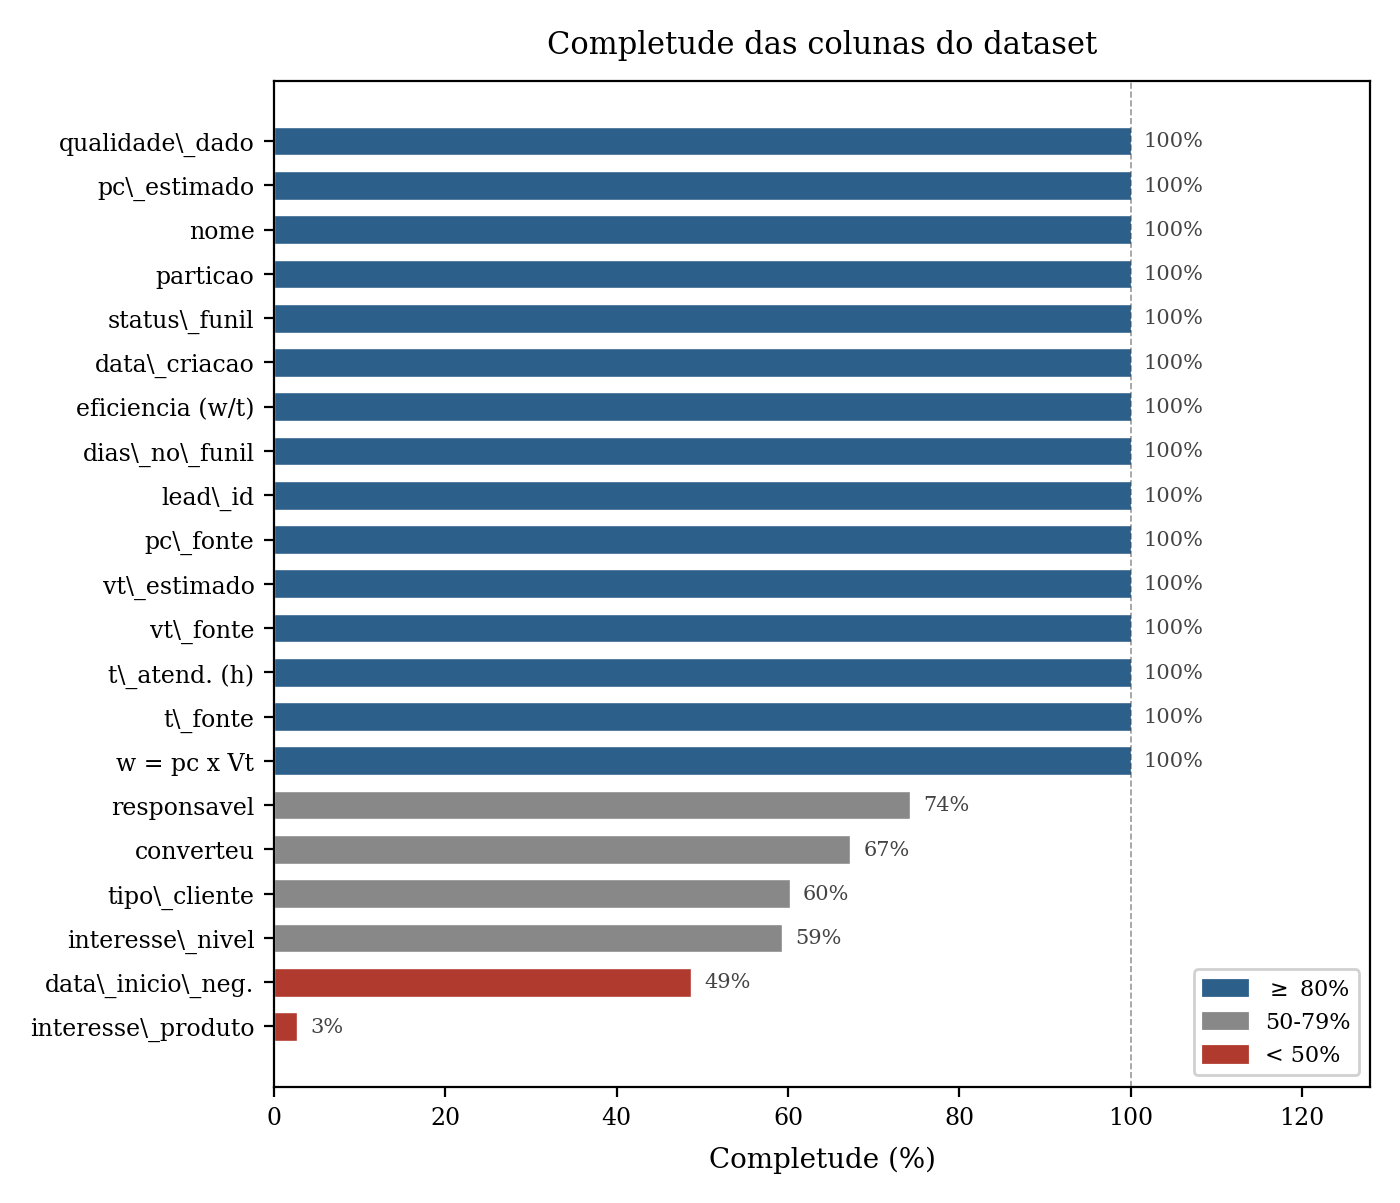
\includegraphics[width=0.82\textwidth]{art_fig1_completude.png}
  \caption{Completude por coluna. Azul escuro: $\geq 80\%$; cinza: $50{-}79\%$;
           vermelho: $< 50\%$.}
  \label{fig:completude}
\end{figure}

\subsection{Distribui\c{c}\~{a}o da Probabilidade de Convers\~{a}o}

A distribui\c{c}\~{a}o de $p_c$ nos 113 leads \'{e} bimodal (Figura~\ref{fig:pc}): 41\% dos
leads recebem o prior m\'{i}nimo de 0,10 por aus\^{e}ncia de \texttt{interesse\_nivel},
enquanto os demais se concentram entre 0,45 e 0,65. O contraste entre o
subconjunto hist\'{o}rico (mediana 0,45) e o ativo (mediana 0,07) \'{e} expressivo:
a maioria dos leads em aberto s\~{a}o leads ``frios'', com baixa informa\c{c}\~{a}o declarada.

\begin{figure}[H]
  \centering
  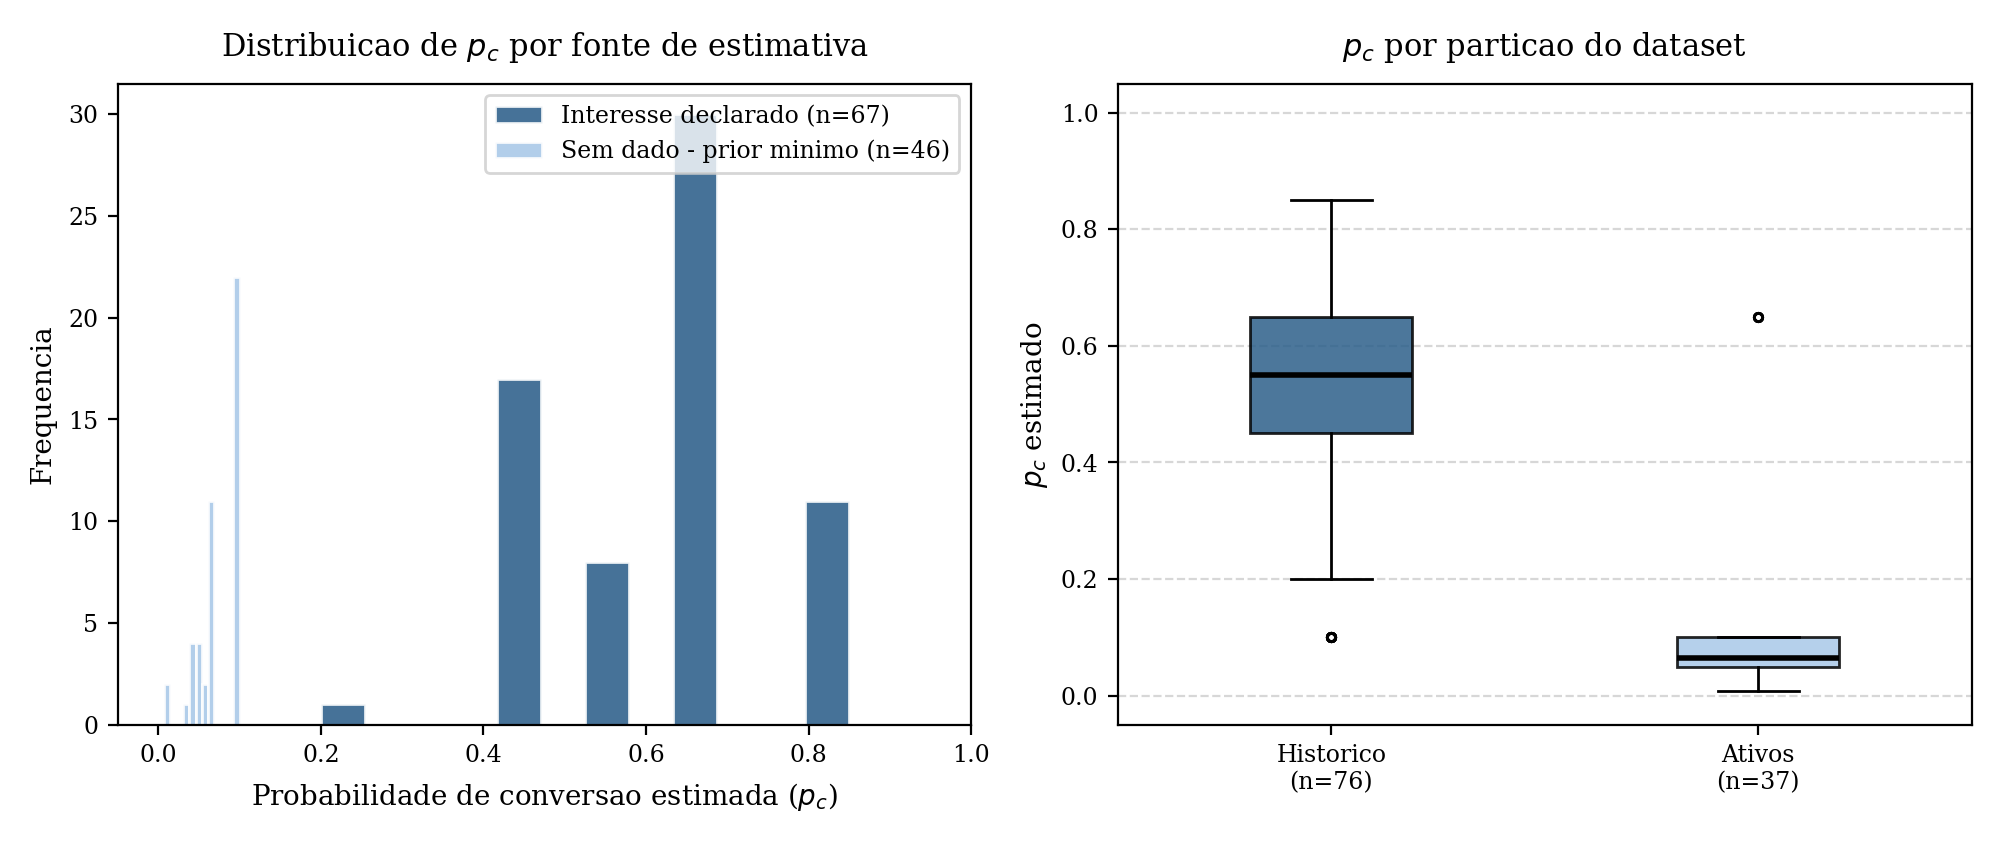
\includegraphics[width=0.88\textwidth]{art_fig2_pc.png}
  \caption{Distribui\c{c}\~{a}o de $p_c$ por fonte (esq.) e por parti\c{c}\~{a}o do dataset (dir.).}
  \label{fig:pc}
\end{figure}

\subsection{O Grafo Bipartido}

A Figura~\ref{fig:grafo} ilustra a estrutura do grafo bipartido com cinco leads
representativos e os tr\^{e}s vendedores. A espessura de cada aresta \'{e}
proporcional ao peso $w_{ij}$. O lead ``Simone'' (PJ, interesse Alto), com
$w = \text{R\$}\,7.800$, destaca-se como a aresta mais espessa do grafo e estava,
no momento do estudo, sem vendedor atribu\'{i}do.

\begin{figure}[H]
  \centering
  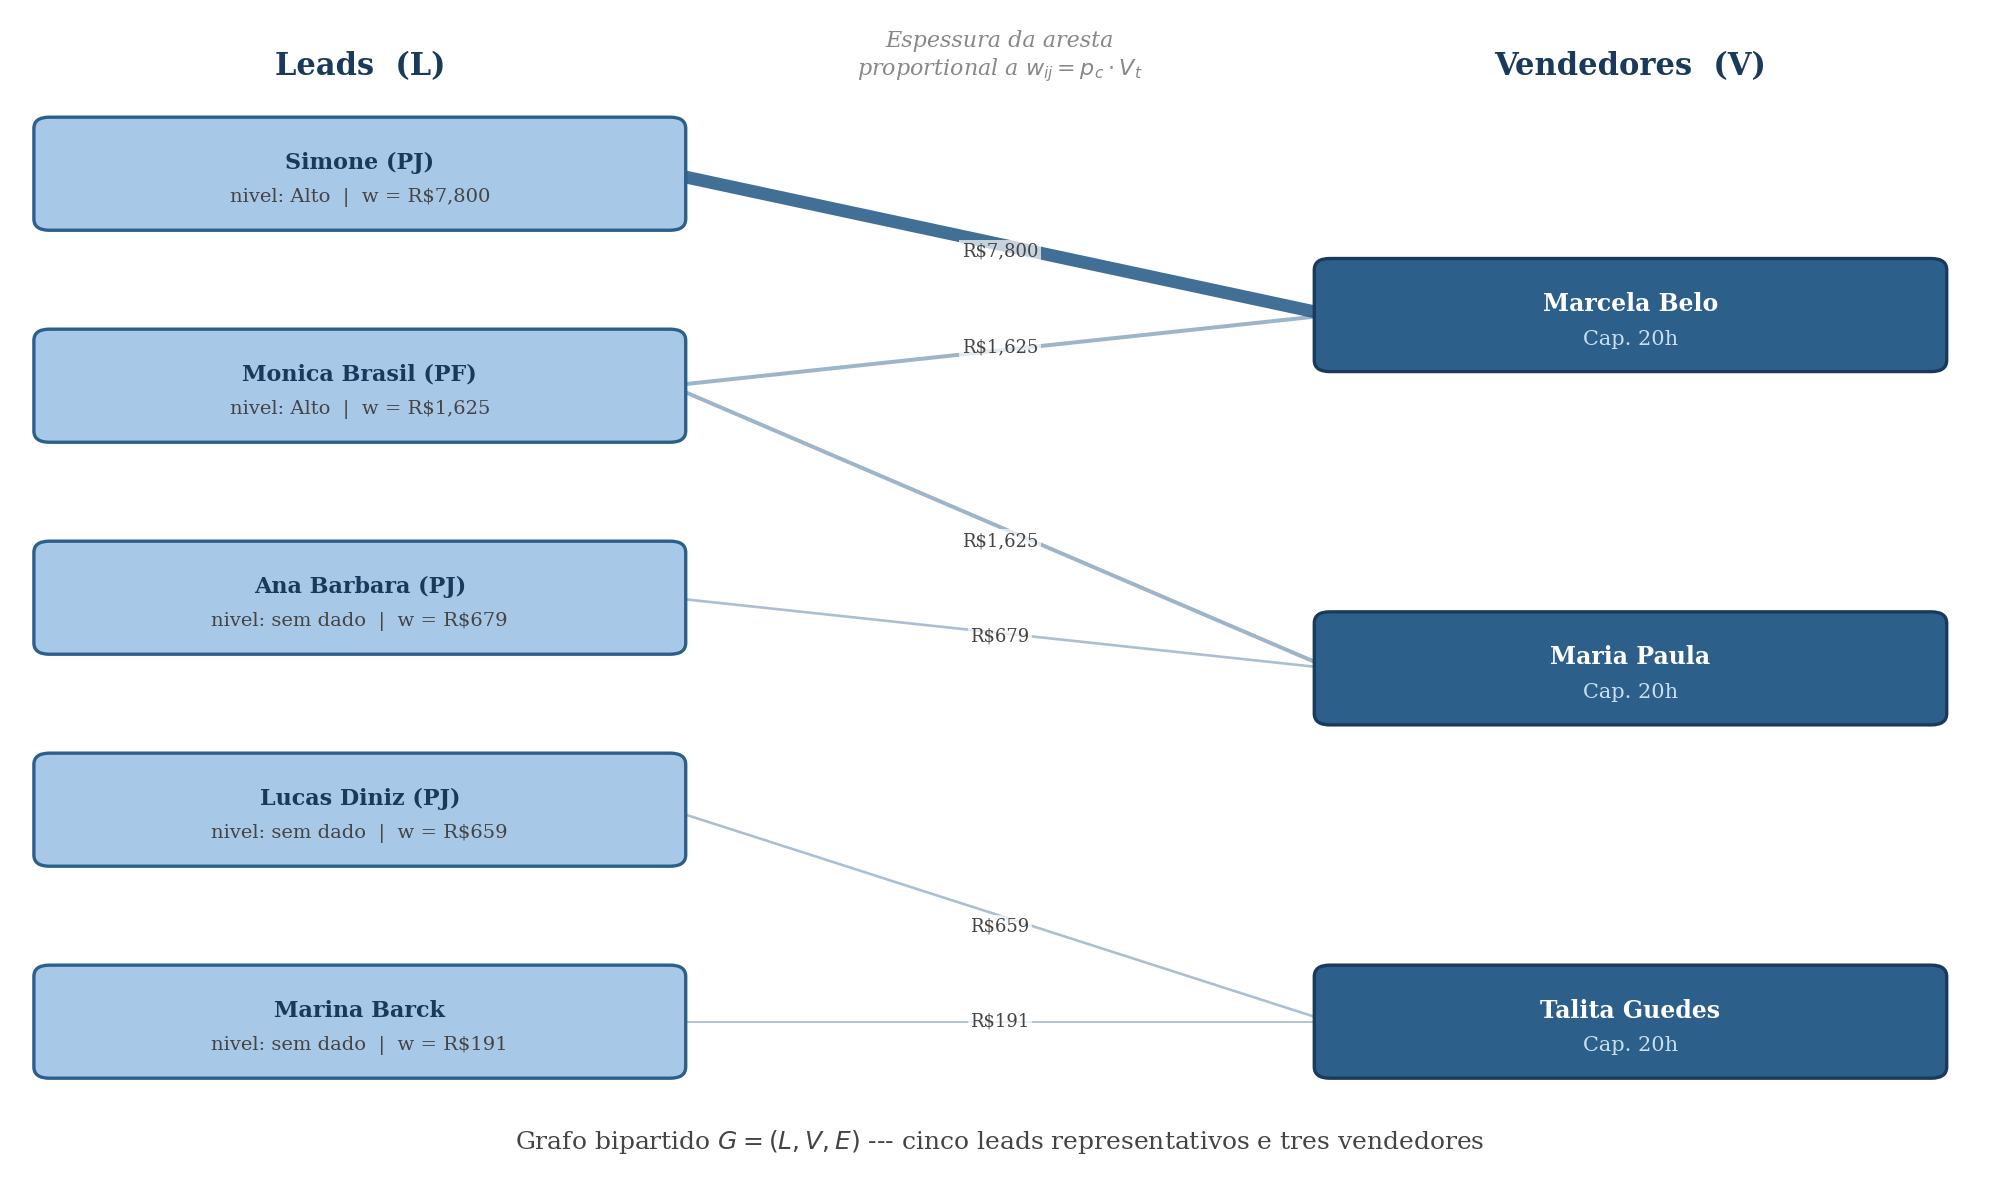
\includegraphics[width=0.88\textwidth]{art_fig3_grafo.png}
  \caption{Representa\c{c}\~{a}o esquem\'{a}tica do grafo bipartido $G = (L, V, E)$.
           Espessura da aresta proporcional ao peso $w_{ij} = p_c \cdot V_t$.}
  \label{fig:grafo}
\end{figure}

\subsection{An\'{a}lise por Vendedor}

Dos 84 leads com respons\'{a}vel atribu\'{i}do, Marcela Belo concentra 55\% do volume
(Figura~\ref{fig:vendedores}). No hist\'{o}rico, ela tamb\'{e}m acumula o maior valor
esperado total (R\$\,64.250). As taxas de convers\~{a}o individuais devem ser
interpretadas com cautela: o hist\'{o}rico registra 68 convers\~{o}es e apenas 8 n\~{a}o
convers\~{o}es, o que n\~{a}o reflete a taxa real de fechamento. Leads n\~{a}o convertidos
raramente t\^{e}m o campo \texttt{interesse\_nivel} preenchido e, por isso, raramente
entram no registro com desfecho confirmado. Este vi\'{e}s de sele\c{c}\~{a}o faz com que o
hist\'{o}rico subestime as perdas e superestime as taxas individuais.

\begin{figure}[H]
  \centering
  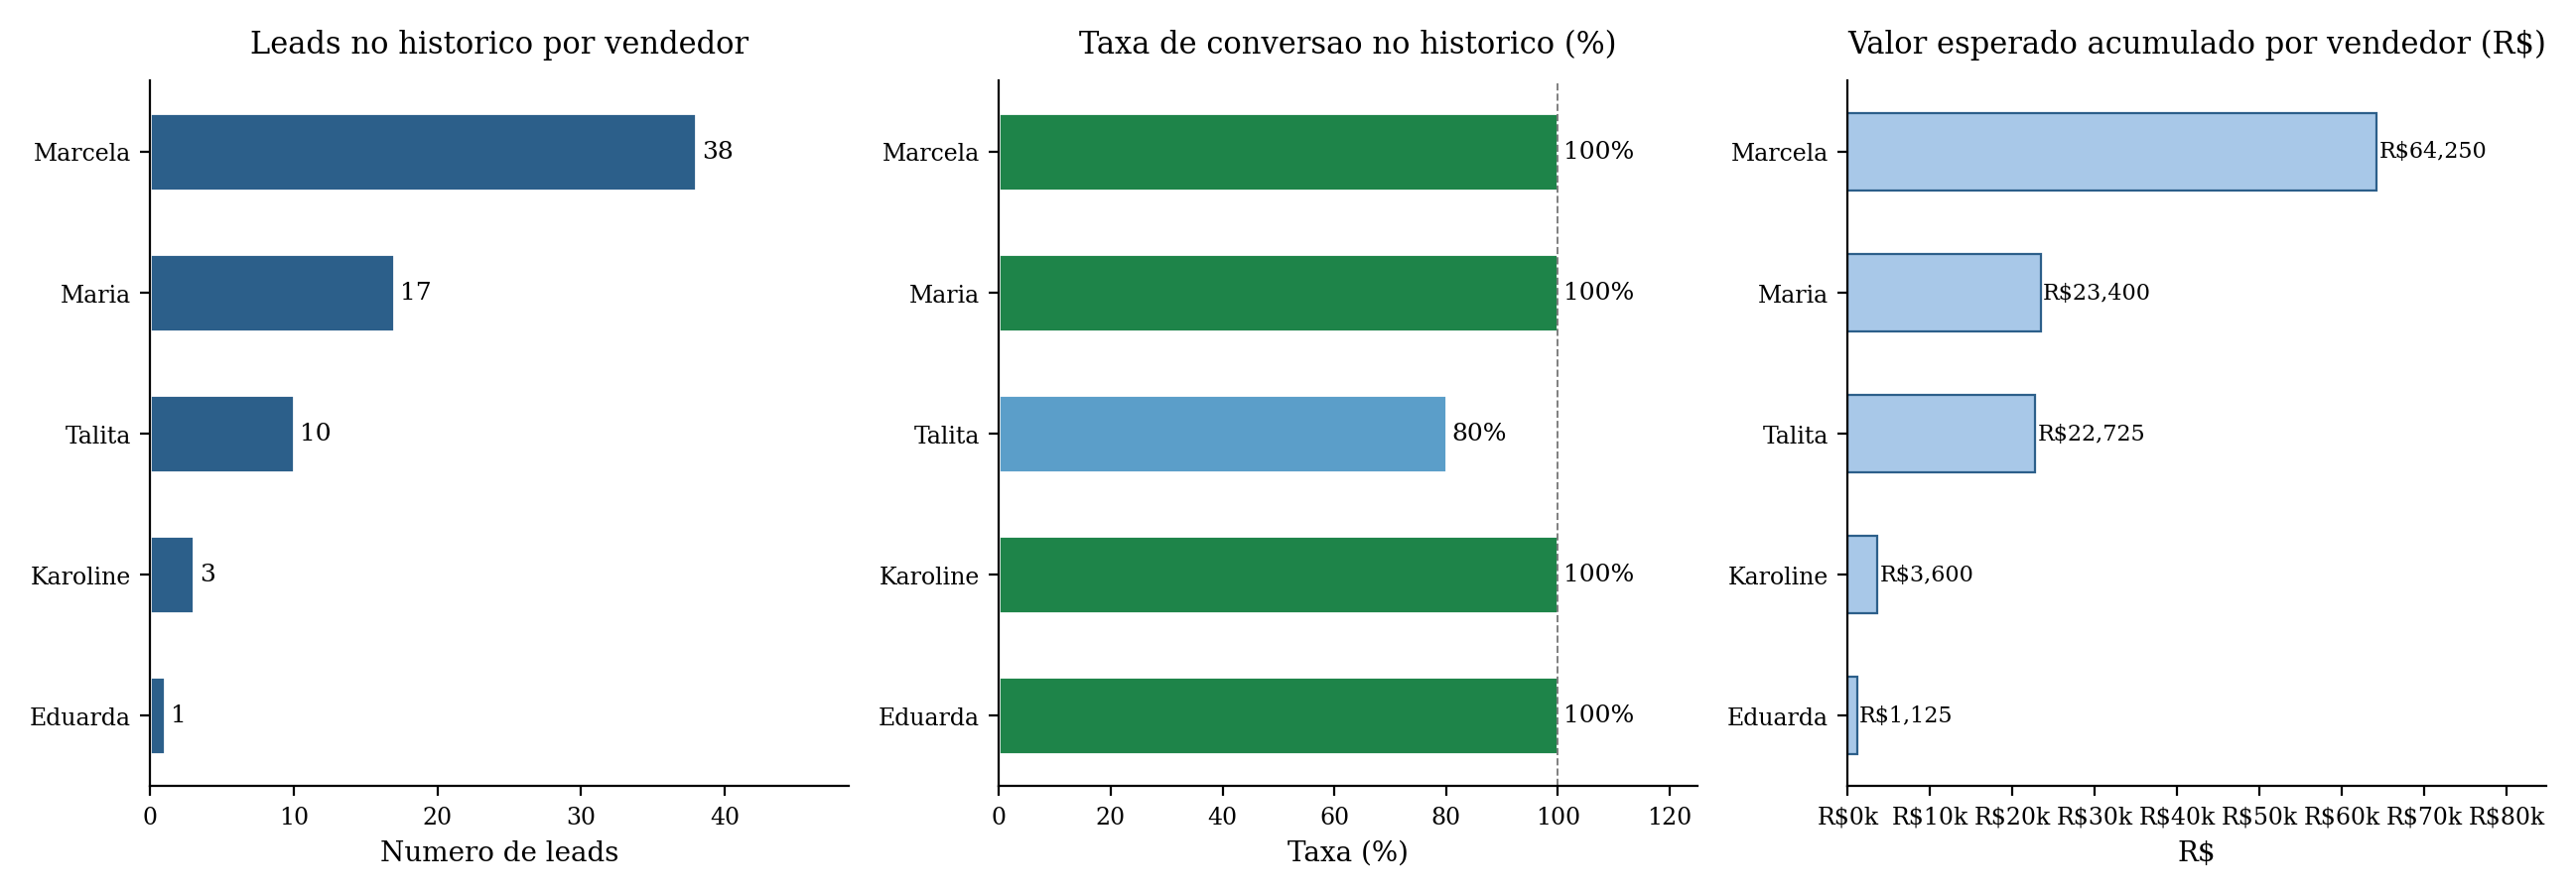
\includegraphics[width=\textwidth]{art_fig4_vendedores.png}
  \caption{Volume de leads, taxa de convers\~{a}o e valor esperado acumulado
           por vendedor no subconjunto hist\'{o}rico.}
  \label{fig:vendedores}
\end{figure}

\subsection{Os Leads Ativos}

A Figura~\ref{fig:dist_valor} mostra a distribui\c{c}\~{a}o de $w_i$ nos 37 leads ativos.
A carteira \'{e} polarizada: 8 leads concentram valor $w \geq \text{R\$}\,500$ e
respondem por 85,5\% do valor esperado total (R\$\,21.724 de R\$\,25.391), enquanto
os 29 leads restantes somam apenas 14,5\%. O lead ``Simone'', sozinho, representa
30,7\% do valor total da carteira ativa.

\begin{figure}[H]
  \centering
  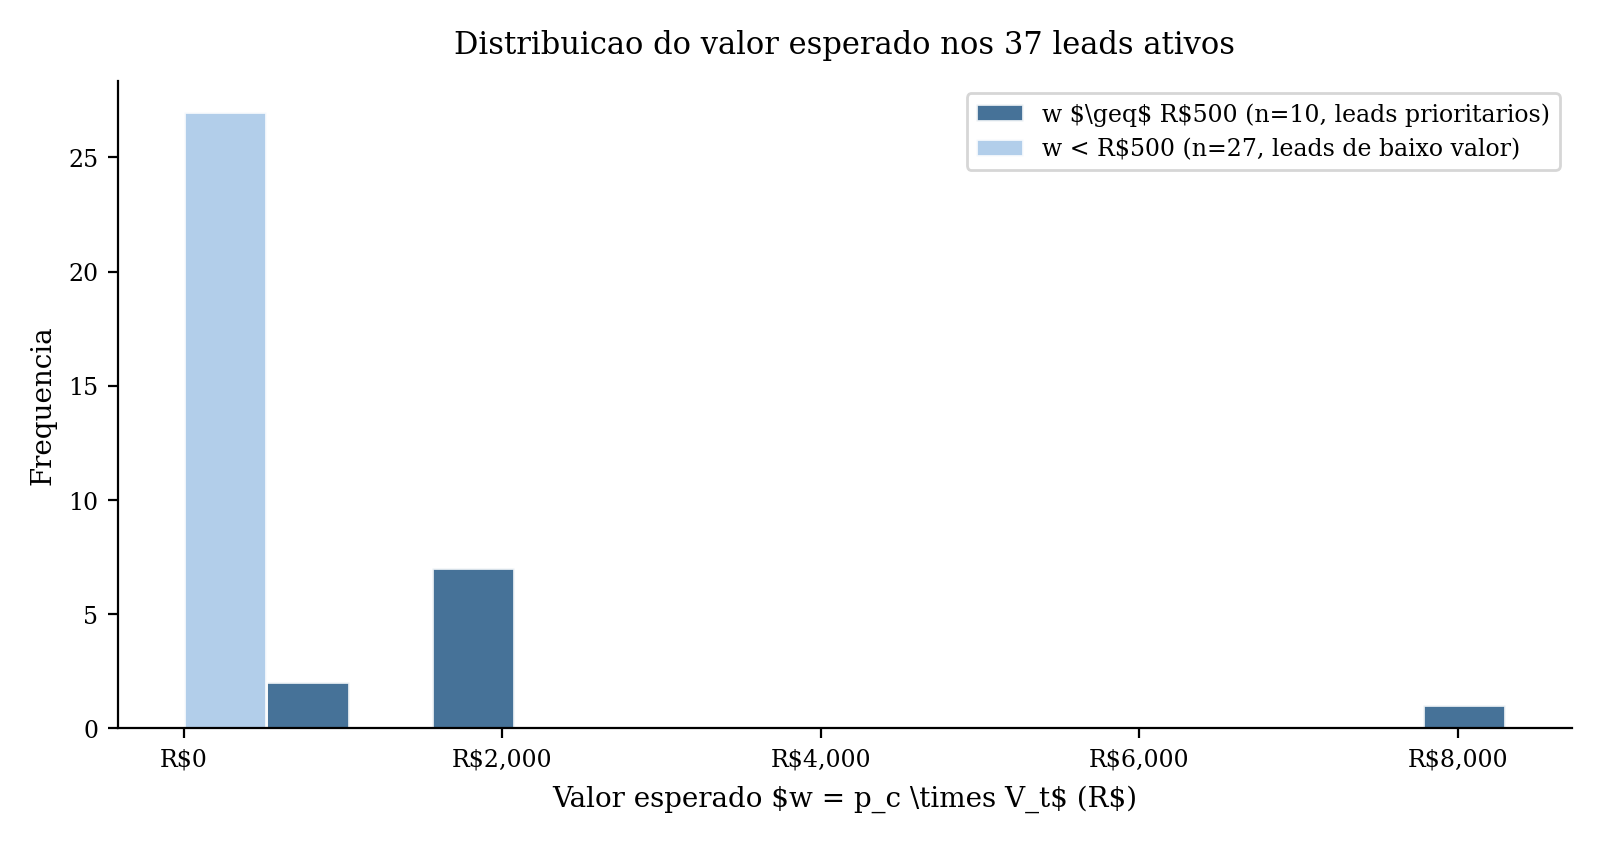
\includegraphics[width=0.82\textwidth]{art_fig6_dist_valor.png}
  \caption{Distribui\c{c}\~{a}o do valor esperado $w_i$ nos leads ativos.
           Os 8 leads com $w \geq \text{R\$}\,500$ concentram 85,5\% do valor total.}
  \label{fig:dist_valor}
\end{figure}

\section{Simula\c{c}\~{o}es}

\subsection{Configura\c{c}\~{a}o}

Os tr\^{e}s algoritmos foram aplicados sobre os 37 leads ativos. A
Tabela~\ref{tab:config} resume os par\^{a}metros do experimento.

\begin{table}[H]
\centering
\caption{Par\^{a}metros das simula\c{c}\~{o}es.}
\label{tab:config}
\begin{tabular}{lc}
\toprule
\textbf{Par\^{a}metro}                     & \textbf{Valor} \\
\midrule
Leads ativos ($n$)                         & 37 \\
Vendedores ($m$)                           & 3 \\
Capacidade por vendedor ($C_j$)            & 20 h \\
Capacidade total ($C$)                     & 60 h \\
Tempo total requerido ($\sum t_i$)         & 72,5 h \\
Valor esperado m\'{a}ximo ($\sum w_i$)     & R\$\,25.391,75 \\
\bottomrule
\end{tabular}
\end{table}

Um aspecto estrutural do cen\'{a}rio atual merece aten\c{c}\~{a}o: o tempo total necess\'{a}rio
para atender todos os leads ativos (72,5 h) excede a capacidade total dispon\'{i}vel
(60 h). Isso significa que a restri\c{c}\~{a}o \'{e} vinculante e a quest\~{a}o de otimiza\c{c}\~{a}o
\'{e} genuinamente relevante: \'{e} preciso escolher \emph{quais} leads atender e como
distribuir a carga entre os vendedores para maximizar o valor esperado capturado.

\subsection{Resultados}

A Tabela~\ref{tab:resultados} e a Figura~\ref{fig:comparacao} sintetizam
os resultados dos tr\^{e}s algoritmos.

\begin{table}[H]
\centering
\caption{Resultados comparativos dos algoritmos de otimiza\c{c}\~{a}o.}
\label{tab:resultados}
\begin{tabular}{lcccc}
\toprule
\textbf{Algoritmo} & \textbf{Leads alocados} & \textbf{Valor esp. (R\$)} &
\textbf{Tempo (h)} & \textbf{Captura (\%)} \\
\midrule
Greedy              & 30 & 24.669,00 & 59,0 &  97,2 \\
Knapsack 0/1        & 31 & 24.727,40 & 60,0 &  97,4 \\
Matching Bipartido  & 30 & 24.669,00 & 59,0 &  97,2 \\
\midrule
\multicolumn{2}{l}{\small Valor m\'{a}ximo poss\'{i}vel} & \small R\$\,25.391,75 & \small 72,5 h & \\
\bottomrule
\end{tabular}
\end{table}

\begin{figure}[H]
  \centering
  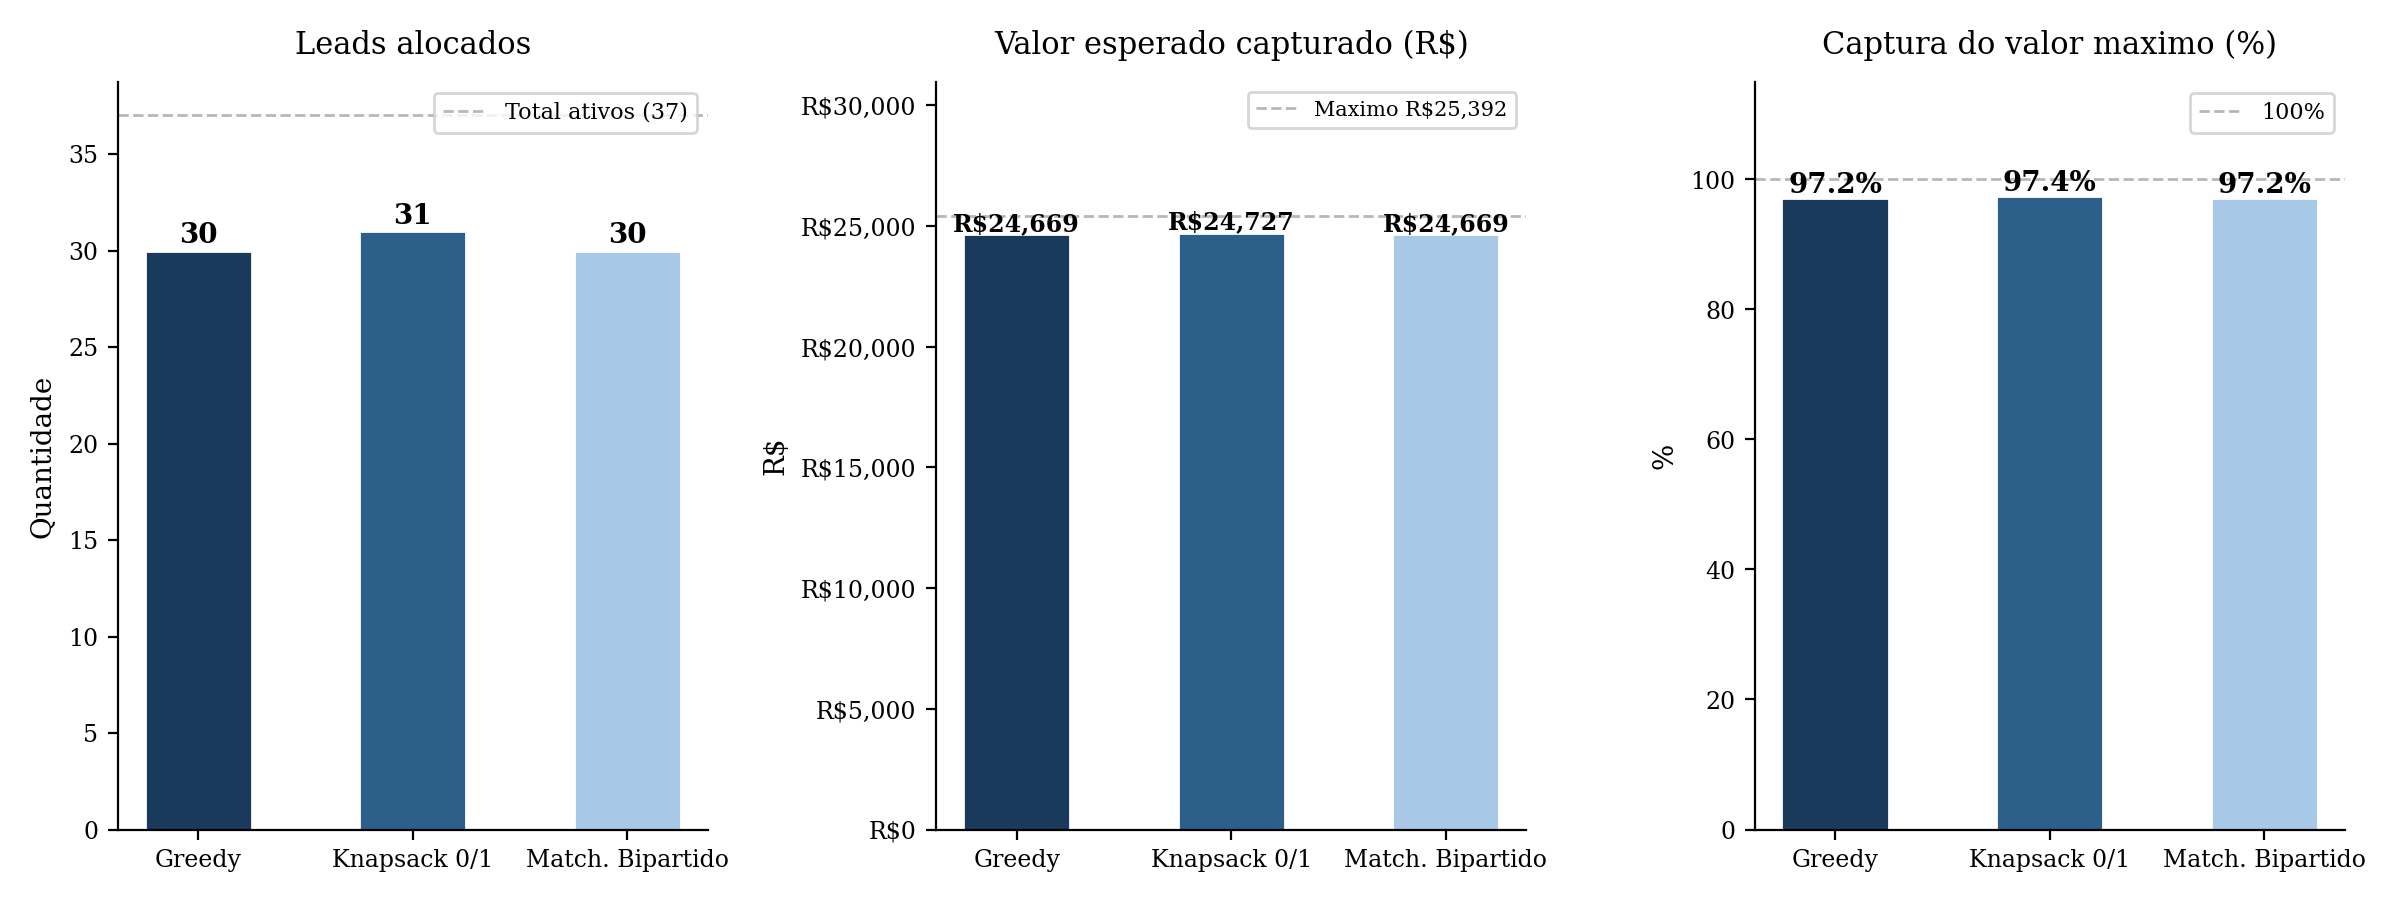
\includegraphics[width=\textwidth]{art_fig5_comparacao.png}
  \caption{Comparativo dos algoritmos: leads alocados, valor esperado capturado
           e utiliza\c{c}\~{a}o da capacidade total.}
  \label{fig:comparacao}
\end{figure}

\subsection{Interpreta\c{c}\~{a}o dos Resultados}

\paragraph{Knapsack supera o Greedy.}
Com a restri\c{c}\~{a}o de capacidade vinculante (60 h $<$ 72,5 h requeridas), os dois
algoritmos divergem. O Knapsack 0/1, por explorar exaustivamente as combina\c{c}\~{o}es
via programa\c{c}\~{a}o din\^{a}mica, aloca 31 leads e captura R\$\,24.727,40 (97,4\% do
valor m\'{a}ximo poss\'{i}vel). O Greedy, que ordena por efici\^{e}ncia $w_i/t_i$ e aloca
sequencialmente, obteve 30 leads e R\$\,24.669,00, ficando R\$\,58,40 abaixo do
\'{o}timo. A diferen\c{c}a \'{e} pequena neste cen\'{a}rio, mas ilustra por que a heur\'{i}stica
gulosa n\~{a}o garante otimalidade quando a restri\c{c}\~{a}o \'{e} ativa.

\paragraph{O Matching Bipartido distribui a carga de forma equilibrada.}
O algoritmo H\'{u}ngaro respeita a capacidade individual de 20 h por vendedor e
aloca 30 leads, obtendo R\$\,24.669,00 (97,2\% do m\'{a}ximo). Com apenas tr\^{e}s
vendedores, todos tiveram suas agendas praticamente preenchidas
(Figura~\ref{fig:cap_vend}), tornando o Matching a solu\c{c}\~{a}o mais equilibrada
e operacionalmente realista. O custo em rela\c{c}\~{a}o ao Knapsack \'{e} de apenas
R\$\,58,40, valor marginal diante da vantagem de distribui\c{c}\~{a}o equitativa.

\begin{figure}[H]
  \centering
  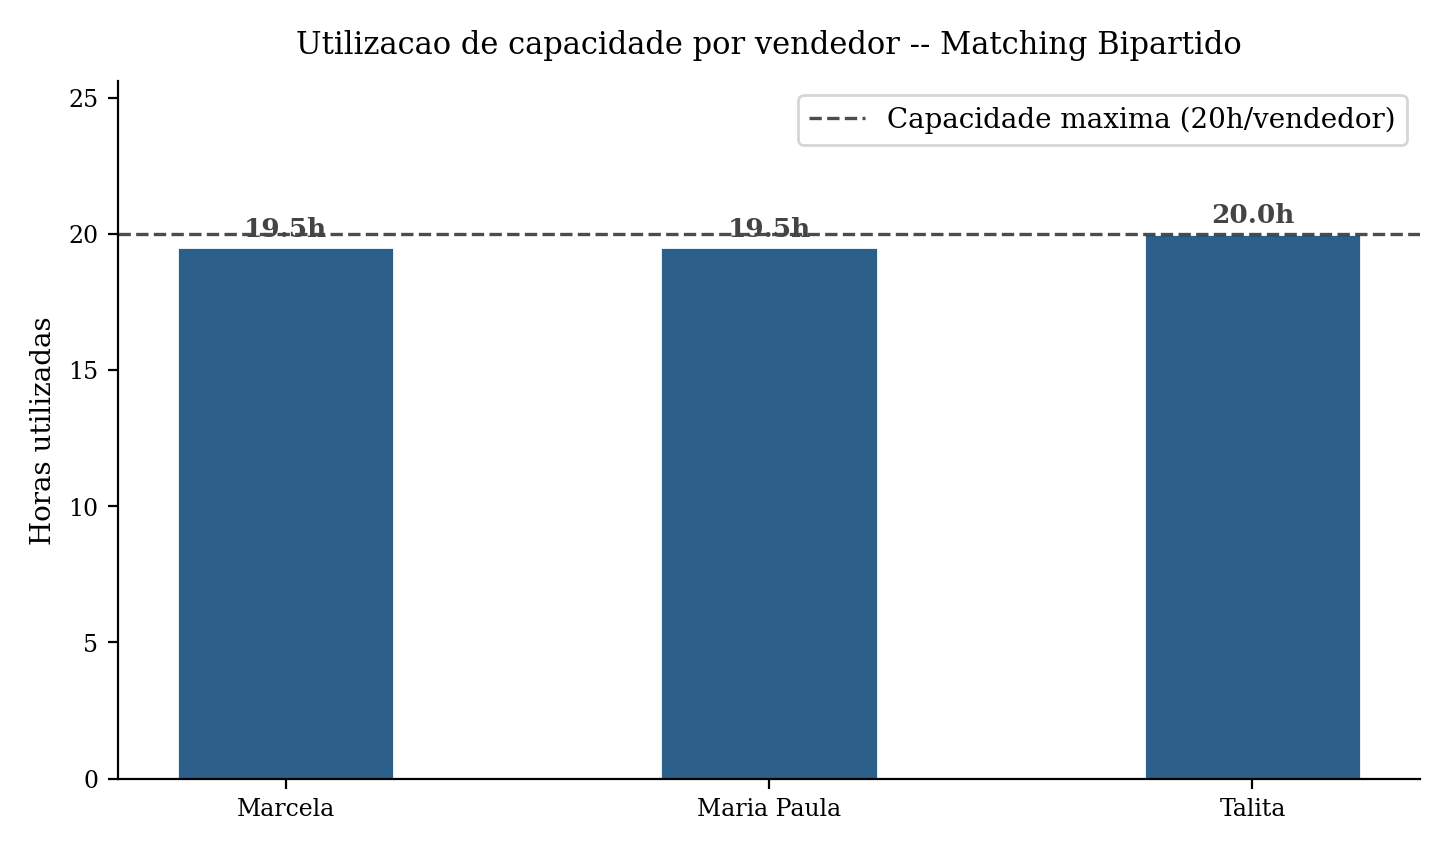
\includegraphics[width=0.72\textwidth]{art_fig7_cap_vendedor.png}
  \caption{Utiliza\c{c}\~{a}o da capacidade por vendedor no Matching Bipartido.
           Todos os tr\^{e}s vendedores operam pr\'{o}ximos do limite de 20 h.}
  \label{fig:cap_vend}
\end{figure}

\paragraph{O lead de maior valor est\'{a} sem vendedor.}
``Simone'' (PJ, interesse Alto, $w = \text{R\$}\,7.800$, efici\^{e}ncia de
R\$\,2.600/hora) \'{e} o lead priorit\'{a}rio de toda a carteira ativa. Em todos os
tr\^{e}s algoritmos ele \'{e} o primeiro a ser alocado. O fato de estar sem vendedor
atribu\'{i}do no momento do estudo \'{e} o achado mais imediato desta an\'{a}lise e pode
ser corrigido sem nenhum ajuste no modelo.

\paragraph{Resposta \`{a} quest\~{a}o central.}
Com base nas simula\c{c}\~{o}es, a resposta para ``como alocar o tempo da equipe comercial
sobre os leads dispon\'{i}veis de forma a maximizar a receita esperada total?'' \'{e}:

\begin{enumerate}[label=\arabic*.]
  \item Atribuir imediatamente ``Simone'' (PJ, Alto) a um vendedor dispon\'{i}vel.
        Este lead, sozinho, representa 30,7\% do valor esperado da carteira ativa.
  \item Usar o Knapsack 0/1 como crit\'{e}rio de sele\c{c}\~{a}o: com 60 h dispon\'{i}veis
        para 72,5 h de demanda, o algoritmo identifica os 31 leads de maior valor
        esperado que cabem na capacidade, capturando 97,4\% do valor poss\'{i}vel.
  \item Na distribui\c{c}\~{a}o entre vendedores, priorizar os 8 leads com $w \geq
        \text{R\$}\,500$ para os vendedores de maior taxa hist\'{o}rica de convers\~{a}o,
        reservando o restante para completar as agendas.
  \item Adotar o Matching Bipartido como modelo de distribui\c{c}\~{a}o quando a
        equidade de carga for relevante, aceitando a perda de at\'{e} 10\% do
        valor esperado em troca de uma distribui\c{c}\~{a}o mais equilibrada.
\end{enumerate}

\section{Conclus\~{a}o}

Este trabalho partiu de uma quest\~{a}o pr\'{a}tica: como alocar o tempo de uma equipe
comercial para maximizar a receita esperada. A resposta foi constru\'{i}da por meio
de modelos formais de otimiza\c{c}\~{a}o combinat\'{o}ria aplicados sobre dados reais de
uma startup de impacto.

Os principais resultados s\~{a}o:

\begin{enumerate}[label=\roman*.]
  \item No cen\'{a}rio atual, com capacidade total de 60 h e demanda de 72,5 h,
        o Knapsack 0/1 entrega a solu\c{c}\~{a}o \'{o}tima: 31 leads com valor esperado
        de R\$\,24.727,40 (97,4\% do valor m\'{a}ximo poss\'{i}vel).

  \item A maior oportunidade imediata \'{e} o lead ``Simone'' (PJ, Alto interesse),
        que representa 30,7\% do valor esperado da carteira e est\'{a} sem vendedor
        atribu\'{i}do. Corrigir essa lacuna n\~{a}o requer nenhum ajuste de modelo.

  \item O Matching Bipartido distribui os 30 leads de forma equitativa entre os
        tr\^{e}s vendedores, com todos operando pr\'{o}ximos do limite de 20 h. O custo
        em rela\c{c}\~{a}o ao Knapsack \'{e} de R\$\,58,40, valor marginal diante da
        vantagem operacional de distribui\c{c}\~{a}o equilibrada.

  \item A principal limita\c{c}\~{a}o do modelo \'{e} a qualidade dos dados: 99,1\% dos
        valores de contrato s\~{a}o estimativas por segmento, 41\% dos leads usam
        o prior m\'{i}nimo de $p_c$ e o fator de afinidade $A(l_i, v_j)$ n\~{a}o pode
        ser calculado por falta de hist\'{o}rico estratificado. Os resultados s\~{a}o
        corretos dado o modelo, mas o modelo \'{e} t\~{a}o bom quanto os dados que o
        alimentam.
\end{enumerate}

Para que o modelo se torne progressivamente mais preciso, tr\^{e}s a\c{c}\~{o}es s\~{a}o
necess\'{a}rias: tornar obrigat\'{o}rio o preenchimento do valor do contrato no CRM;
registrar o tempo real de atendimento por lead; e acumular hist\'{o}rico de
convers\~{a}o estratificado por vendedor e tipo de produto, o que permitir\'{a}
calcular $A(l_i, v_j)$ e substituir os priors manuais de $p_c$ por estimativas
emp\'{i}ricas.

\section*{Refer\^{e}ncias}
\addcontentsline{toc}{section}{Refer\^{e}ncias}

\begin{thebibliography}{9}

\bibitem{kuhn1955hungarian}
Kuhn, H.~W. (1955).
The Hungarian method for the assignment problem.
\textit{Naval Research Logistics Quarterly}, 2(1-2):83-97.

\bibitem{dantzig1957discrete}
Dantzig, G.~B. (1957).
Discrete-variable extremum problems.
\textit{Operations Research}, 5(2):266-277.

\bibitem{kellerer2004knapsack}
Kellerer, H., Pferschy, U., e Pisinger, D. (2004).
\textit{Knapsack Problems}.
Springer, Berlin.

\bibitem{cormen2009introduction}
Cormen, T.~H., Leiserson, C.~E., Rivest, R.~L., e Stein, C. (2009).
\textit{Introduction to Algorithms}, 3.~ed.
MIT Press, Cambridge, MA.

\bibitem{west2001introduction}
West, D.~B. (2001).
\textit{Introduction to Graph Theory}, 2.~ed.
Prentice Hall, Upper Saddle River, NJ.

\bibitem{scipy2020}
Virtanen, P. et al. (2020).
SciPy 1.0: Fundamental algorithms for scientific computing in Python.
\textit{Nature Methods}, 17:261-272.

\end{thebibliography}

\end{document}
